\section{Durchführung}
\label{sec:Durchfuehrung}
Ein quecksilberbedampftes Glasrohr befindet sich in einem heizbaren Blechgehäuse. Die Temperatur $T$ kann über einen Regler eingestellt und konstant gehalten werden. In dem Glasrohr befinden sich ein Heizdraht, sowie Beschleuniger- und Auffängerelektrode.
Der Heizfaden wird über ein Konstantspannungsgerät betrieben, die Elektroden über elektrische Geräte, deren Ausgangsspannung sich zeitproportional ändern kann. 
Die Spannungen können über die Bereiche $0\leq U_\mathup{B} \leq \SI{60}{\volt}$ und $0\leq U_\mathup{A}\leq \SI{11}{\volt}$ variiert werden. Der Auffängerstrom $I_\mathup{A}$ an der Auffängerelektrode wird über ein Picoamperemeter gemessen.
Es besteht aus einem Gleichstromverstärker und Aperemeter, das proportional zum Eingangsstrom ausschlägt. 
Der gesamte Aufbau samt \textsc{Frank}-\textsc{Hertz}-Röhre sind in Abbildung \ref{fig:aufbau} dargestellt.
\begin{figure}
	\centering
	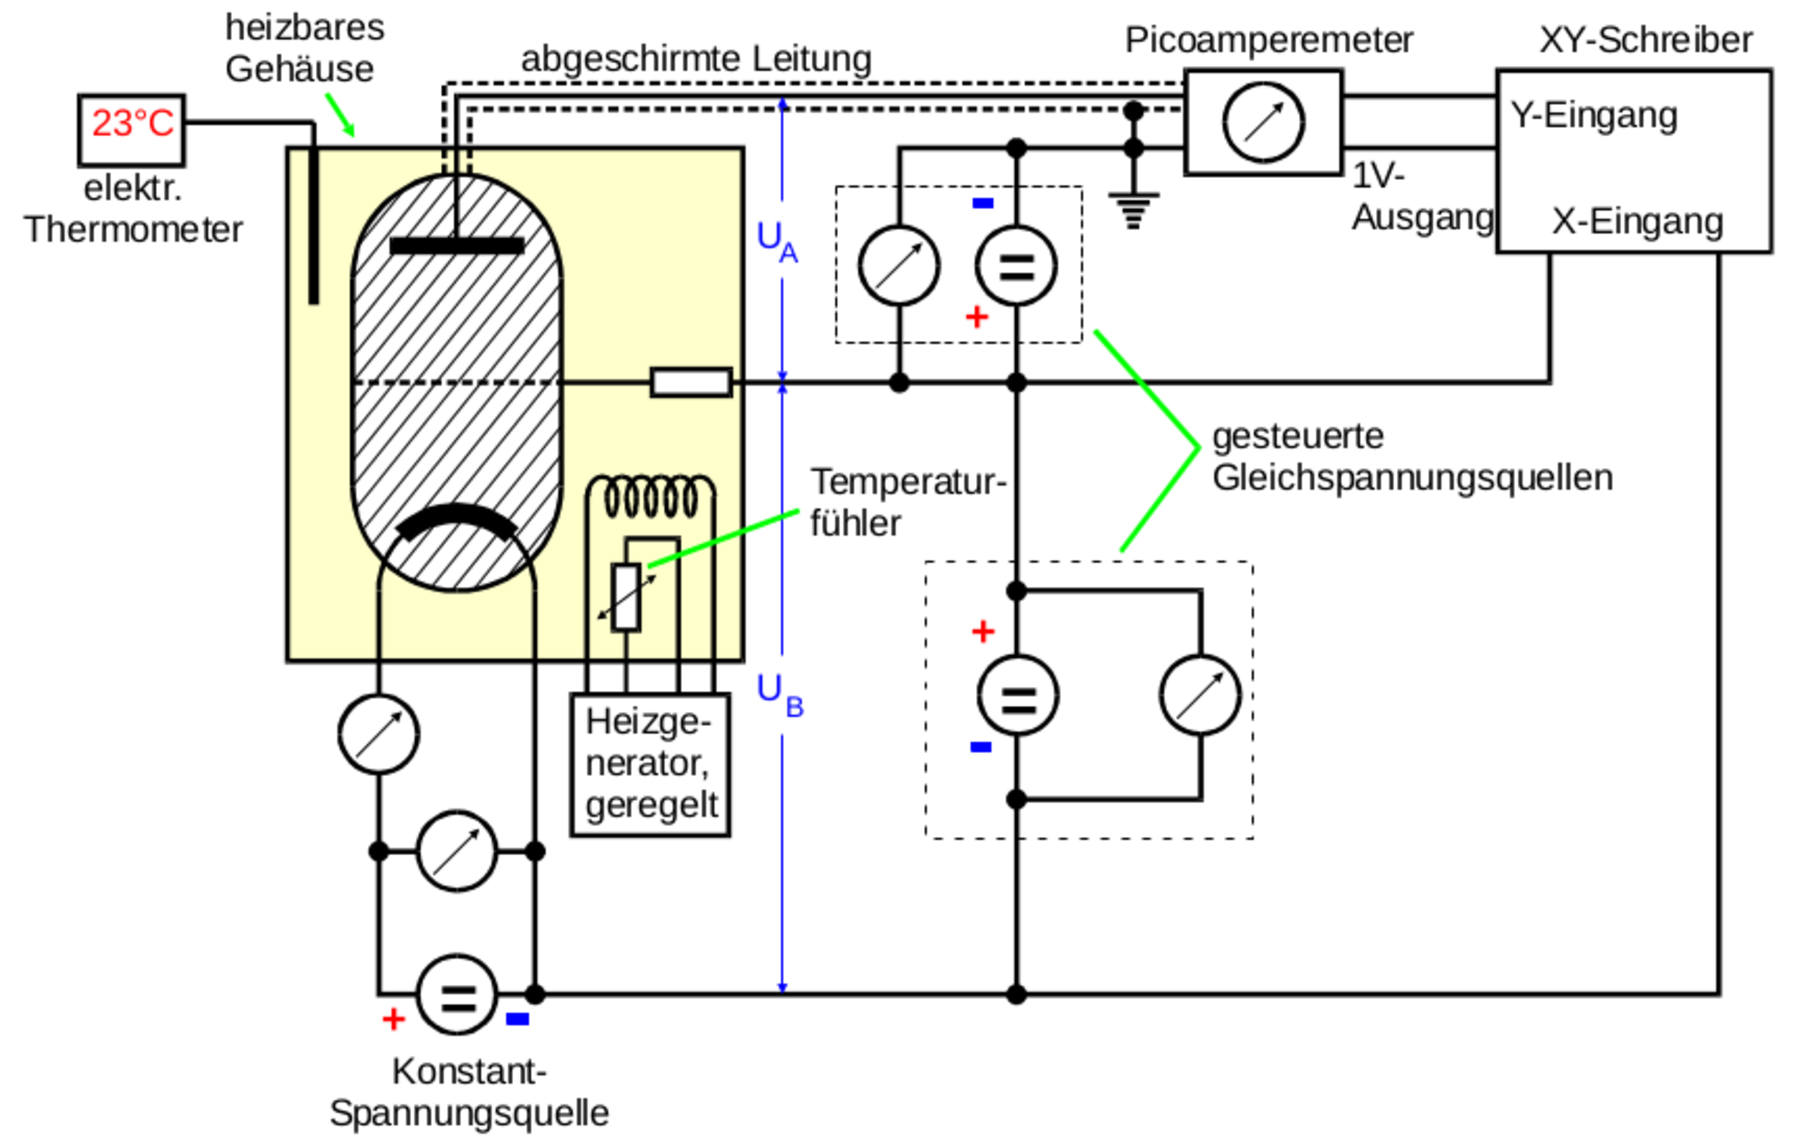
\includegraphics[width=0.8\textwidth]{Bilder/Aufbau_Detail.pdf}
	\caption{Detaillierter Aufbau des Versuches.}
	\label{fig:aufbau}
\end{figure}
\begin{itemize}
\item{Franck-Hertz-Kurve}

Um eine \textsc{Franck}-\textsc{Hertz}-Kurve aufzeichnen zu können wird ein XY-Schreiber genutzt. 
Auf der X-Achse wird $U_\mathup{B}$ aufgetragen, in Y-Richtung eine Spannung $U$ proportional zum Strom $I_\mathup{A}$. 
Diese Spannung wird vom Picoamperemeter geliefert.
Die Justierung des Schreibers erfolgt über die "zero"-Knöpfe. Damit wird der Nullpunkt in die linke untere Ecke gelegt.
Während des Justierens sollte kein Signal an den Eingängen liegen.
Die Empfindlichkeit der Eingänge wird eingestellt, in dem ein geringes Signal angelegt und langsam gesteigert wird. 
Die Auslenkung des Y-Schreibers sollte maximal sein, wenn $I_\mathup{A}\approx \SI{3}{\nano\ampere}$ erreicht.
Die X-Komponente muss vollen Ausschlag zeigen, wenn die Maximalspannung erreicht ist.
Um die Achse auf Volt zu eichen werden einige Werte eingetragen, die vom Voltmeter abgelesen werden.
Der Hg-Dampfdruck wird nach Kapitel \ref{sec:Theorie} eingestellt.
Dafür wird das Blechgehäuse erhitzt bis der Ausgangsstrom ein Maximum von ${2,1-2,2}{\si\ampere}$ erreicht.Die Temperatur $T$ kann abgelesen werden. 
Sobald die gewünschte Temperatur erreicht ist sollte diese heruntergeregelt werden werden, bis der Ausgangsstrom nun ein Minimum von $\SI{1,2}{\ampere}$ erreicht. 
$T$ ist konstant, wenn der Strom zwischen beiden Extremwerten schwingt.
Die Heizleistung des Drahtes sollte so weit gesenkt werden, dass bei $U_\mathup{B}\approx \SI{60}{\volt}$ ein Strom $I_\mathup{A}={1-3}{\si{\nano\ampere}}$ auftritt. 
Die Kurve wird bei Temperaturen, die zwischen ${160-200}\si{\celsius}$ liegen, im Bereich von $0\leq U_\mathup{B} \leq \SI{60}{\volt}$ aufgenommen mit $U_\mathup{A}\approx \SI{1}{\volt}$.
\item{Energieverteilung der Elektronen}

Der Strom $I_\mathup{A}$ wird in Abhängigkeit von der Bremsspannung $U_\mathup{A}$ aufgezeichnet bei einer Beschleunigungsspannung von $U_\mathup{B}=\SI{11}{\volt}$. 
Die Messung wird bei $T\approx \SI{20}{\degree\celsius},T={140-160}{\si\celsius}$ durchgeführt.
FÜr $T\approx \SI{20}{\celsius}$ wird bei $U_\mathup{A}=0$ ein Strom $I_\mathup{A}=\SI{50}{\volt}$ eingestellt, in dem die Kathodenheizung neu eingeregelt wird.
\item{Ionisierungsspannung}

Der Strom $I_\mathup{A}$ wird in Abhängigkeit von $U_\mathup{B}$ aufgenommen. Die Anodenspannung bleibt konstant $U_\mathup{A}=\SI{-30}{\volt}$.
\end{itemize}
